\section{Proposed PHQD Framework}\label{sec:method}

\subsection{Overview}
PHQD removes Gaussian noise from the latent representation of an image, one small patch at a time, so that each patch fits a few-qubit circuit. Figure~\ref{fig:architecture} shows the workflow. A convolutional autoencoder compresses a Fashion-MNIST image into a latent map, Gaussian noise is added, and the noisy map is cut into overlapping patches. A hybrid quantum--classical model denoises each patch, the patches are averaged back into a latent map, an optional stitching network refines it, and the decoder produces the image.

\begin{figure*}[t]
\centering
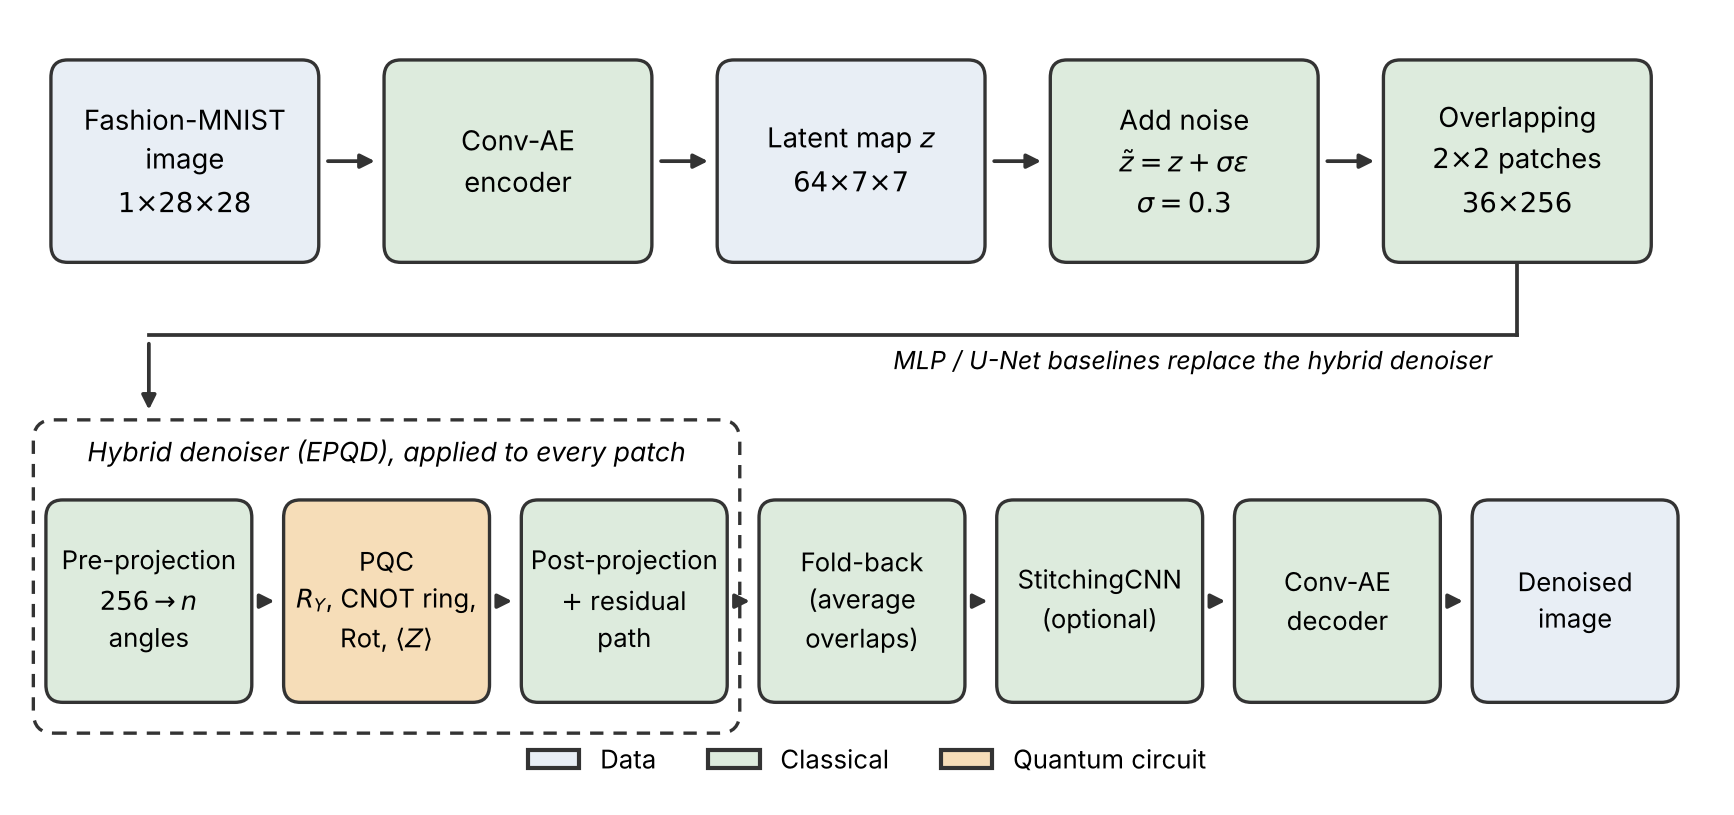
\includegraphics[width=0.92\textwidth]{phqd_architecture.png}
\caption{Overall pipeline of the proposed PHQD framework.}
\label{fig:architecture}
\end{figure*}

\subsection{Data and Preprocessing}
We use Fashion-MNIST~\cite{fmnist} with 60{,}000 training and 10{,}000 test grayscale images of $28\times28$ pixels. Pixels are normalized with mean 0.5 and standard deviation 0.5, so they lie in $[-1,1]$. The encoder of the trained, frozen autoencoder maps each image to a latent map $z\in\mathbb{R}^{64\times7\times7}$, which is corrupted as
\begin{equation}
    \tilde z = z+\sigma\epsilon,\qquad \epsilon\sim\mathcal{N}(0,I),\quad \sigma=0.3.
\end{equation}
A $2\times2$ window with stride one over the $7\times7$ grid gives 36 overlapping patches per image, each flattened to $64\times2\times2=256$ values.

\subsection{Convolutional Autoencoder}
The encoder has two strided convolutions ($1\rightarrow32\rightarrow64$ channels, $4\times4$ kernel, stride 2, padding 1), each followed by batch normalization and LeakyReLU, and maps an image to a $64\times7\times7$ latent map. The decoder mirrors it with two transposed convolutions and a Tanh output. It is trained with MSE loss and Adam (learning rate $10^{-3}$, cosine annealing) for 20 epochs with batch size 128.

\subsection{EPQD Denoiser}
For each patch $p$, a classical pre-projection ($256\rightarrow128\rightarrow n$) with a Tanh output gives $n$ values that are mapped to rotation angles in $[0,\pi]$:
\begin{equation}
    a(p)=\frac{\pi}{2}\left(g_{\mathrm{pre}}(p)+1\right).
\end{equation}
The circuit applies $R_Y(a_i)$ on each of $n$ qubits. Each of $L$ variational layers then applies a ring of CNOT gates followed by a trainable \texttt{Rot} gate on every qubit, and the circuit returns the Pauli-$Z$ expectations
\begin{equation}
    q(p)=\left(\langle Z_0\rangle,\ldots,\langle Z_{n-1}\rangle\right).
\end{equation}
A classical post-projection ($n\rightarrow128\rightarrow256\rightarrow256$) and a learned linear residual path from the input give the denoised patch:
\begin{equation}
    \hat p=g_{\mathrm{post}}(q(p))+W_rp+b_r.
\end{equation}
The circuit is simulated with PennyLane on \texttt{default.qubit} using backpropagation. The IQP variant (EPQD-IQP) replaces the first step with Hadamard gates, data-dependent $R_Z$ rotations and Ising-$ZZ$ interactions. Table~\ref{tab:configs} lists the four 4-qubit configurations.

\begin{table}[t]
\centering
\caption{Standard EPQD quantum configurations.}
\label{tab:configs}
\begin{tabular}{lccc}
\toprule
\textbf{Model} & \textbf{Qubits} & \textbf{Layers} & \textbf{Ansatz}\\
\midrule
EPQD-S & 4 & 1 & Basic ring + Rot\\
EPQD-M & 4 & 2 & Basic ring + Rot\\
EPQD-L & 4 & 3 & Basic ring + Rot\\
EPQD-IQP & 4 & 2 & IQP-style + ring + Rot\\
\bottomrule
\end{tabular}
\end{table}

\subsection{EPQD-6Q-V2}
EPQD-6Q-V2 uses six qubits and three layers, re-uploads the input in every layer, and reads out $X$, $Y$ and $Z$ on each qubit, which gives 18 features for the post-projection:
\begin{equation}
    q_{\mathrm{XYZ}}\in\mathbb{R}^{18}.
\end{equation}
It is trained jointly with the stitching network using the loss
\begin{equation}
    \mathcal{L}_{\mathrm{V2}}=
    \mathcal{L}_{\mathrm{latent\text{-}MSE}}
    +0.5\,\mathcal{L}_{\mathrm{image\text{-}MSE}}
    +0.2\left(1-\operatorname{SSIM}(\hat x,x)\right).
\end{equation}

\subsection{Stitching Network and Fold-Back}
Denoised patches are placed back at their grid positions, and overlapping estimates are averaged:
\begin{equation}
    \hat z(c,h,w)=
    \frac{1}{|\mathcal{I}(h,w)|}\sum_{p\in\mathcal{I}(h,w)}\hat p(c,h-h_p,w-w_p),
\end{equation}
where $\mathcal{I}(h,w)$ is the set of patches covering position $(h,w)$. The optional StitchingCNN is a classical network (a $1\times1$ stem, three residual blocks with two $3\times3$ convolutions each, and a $1\times1$ Tanh head with a skip connection) that refines this map. It is first trained alone to remove noise with standard deviation 0.15 from latent maps, for 15 epochs with Adam at $10^{-3}$. The decoder then turns the latent map into the denoised image.

\subsection{Training}
The standard EPQD models are trained in two stages with MSE loss, Adam, cosine annealing and batch size 128. In the warm-up, the quantum weights are frozen and a linear bypass replaces the circuit, so that the classical layers train for 10 epochs at learning rate $10^{-3}$. The bypass is then removed and the whole model is fine-tuned for 8 epochs at $3\times10^{-3}$ on at most 8{,}000 patches. EPQD-6Q-V2 uses three phases of 15, 8 and 6 epochs with learning rates $10^{-3}$, $2\times10^{-3}$ and $5\times10^{-4}$, the last one jointly with the stitching network.

\subsection{Baselines and Evaluation}
The MLP baseline denoises flattened 256-value patches ($256\rightarrow512\rightarrow512\rightarrow256\rightarrow256$ with LayerNorm, GELU, dropout 0.1 and a residual connection). The U-Net baseline denoises the full $64\times7\times7$ latent map with two encoder blocks (64 and 128 channels), a 256-channel bottleneck and a decoder with skip connections. Both are trained for 20 epochs with MSE loss, Adam at $10^{-3}$ and batch size 128. All denoisers receive the same noisy latent maps with $\sigma=0.3$, and the decoded clean and noisy latent maps serve as upper and lower references.

We report MSE, PSNR $=10\log_{10}(1/\mathrm{MSE})$ and SSIM between the decoded and original images mapped to $[0,1]$ on test images, and the Fr\'echet Inception Distance (FID) from Inception-V3 features of 1{,}000 test images. Lower MSE and FID and higher PSNR and SSIM are better.
